\documentclass[10pt]{article}

\usepackage{graphicx}
\usepackage{amsmath}
\usepackage{algorithm}
\usepackage{algpseudocode}
\usepackage{tikz}
\usepackage{hyperref}
\usepackage{booktabs}
\usepackage{listings}
\usepackage{float}
\usepackage{microtype}
\lstset{
    basicstyle=\small\ttfamily,
    breaklines=true,
    breakatwhitespace=true,
    showstringspaces=false,
    columns=flexible
}

\begin{document}

\title{NEXUS: A High-Performance Collision Detection System for Interactive Image Annotation}

\author{Technical Documentation Team\\
YipYap Project\\

\includegraphics[width=0.5cm]{favicon.pdf}}

\maketitle

\begin{abstract}
We present NEXUS (Network of Efficiently Cross-referenced Unified Spatial-groups), a collision detection and box cycling system optimized for interactive image annotation applications. NEXUS applies established Union-Find algorithms with Axis-Aligned Bounding Box (AABB) collision detection to provide real-time overlap detection and intuitive cycling through overlapping bounding boxes. Our system achieves sub-3ms response times for typical annotation scenarios through strategic caching and optimization techniques, making it particularly suitable for production applications requiring real-time user interaction with multiple overlapping annotations.
\end{abstract}

\section{Introduction}
Modern image annotation systems frequently require users to interact with multiple overlapping bounding boxes, presenting challenges in both computational efficiency and user experience. While connected components analysis for geometric objects is well-established in computational geometry, existing annotation tools often lack efficient mechanisms for navigating overlapping regions in real-time interactive contexts. NEXUS addresses these practical challenges through optimized implementation of established algorithms combined with intuitive user interface design.

\section{System Architecture}
\subsection{Core Components}
NEXUS consists of five main subsystems:
\begin{enumerate}
    \item Input Processing
    \item Collision Detection
    \item Union-Find Algorithm
    \item Group Processing
    \item Box Cycling
\end{enumerate}

\subsection{Mathematical Foundation}
The system's collision detection is based on the Separating Axis Theorem (SAT) simplified for axis-aligned bounding boxes (AABB). Bounding boxes are represented by their top-left corner, $(x_1, y_1)$, and their bottom-right corner, $(x_2, y_2)$.

For two boxes, A and B, an overlap occurs if and only if their projections on both the x and y axes overlap. This is determined by the following condition:

\begin{equation}
\begin{split}
    \text{overlap}(A, B) = & (A.x_1 \leq B.x_2) \land \\
    & (B.x_1 \leq A.x_2) \land \\
    & (A.y_1 \leq B.y_2) \land \\
    & (B.y_1 \leq A.y_2)
\end{split}
\end{equation}

This approach ensures efficient and accurate collision detection, forming the basis for identifying connected components of overlapping annotations.

\section{Algorithmic Implementation}
\subsection{Union-Find Data Structure}
The core of NEXUS is a modified Union-Find data structure with path compression and union by rank optimizations. The time complexity for find and union operations is $O(\alpha(n))$, where $\alpha(n)$ is the inverse Ackermann function.

\begin{algorithm}
\caption{Union-Find with Path Compression and Union by Rank}
\begin{algorithmic}[1]
\Function{Find}{x}
    \If{parent[x] $\neq$ x}
        \State parent[x] $\gets$ Find(parent[x]) \Comment{Path Compression}
    \EndIf
    \Return parent[x]
\EndFunction
\Statex
\Function{Union}{x, y}
    \State rootX $\gets$ Find(x)
    \State rootY $\gets$ Find(y)
    \If{rootX $\neq$ rootY}
        \If{rank[rootX] < rank[rootY]} \Comment{Union by Rank}
            \State parent[rootX] $\gets$ rootY
        \ElsIf{rank[rootX] > rank[rootY]}
            \State parent[rootY] $\gets$ rootX
        \Else
            \State parent[rootY] $\gets$ rootX
            \State rank[rootX] $\gets$ rank[rootX] + 1
        \EndIf
    \EndIf
\EndFunction
\end{algorithmic}
\end{algorithm}

\subsection{Spatial Caching}
NEXUS implements a sophisticated caching system with the following properties:
\begin{itemize}
    \item Cache duration: 100ms
    \item Cache invalidation based on box property hashing
    \item Flat cache structure storing the latest computed overlap groups
\end{itemize}

\subsection{Component Extraction}
The `getComponents()` method efficiently extracts all connected components from the Union-Find data structure in a single pass. The algorithm operates as follows:

\begin{enumerate}
    \item Initialize an empty map, `components`, where keys are the root indices of each component and values are lists of the indices of their members.
    \item Iterate through each element `i` from `0` to `n-1`, where `n` is the total number of elements.
    \item For each element `i`, find its root `r` by calling the `find(i)` operation.
    \item Check if `r` exists as a key in the `components` map.
    \begin{itemize}
        \item If `r` is not in the map, add it with a new list containing `i`.
        \item If `r` is already in the map, append `i` to the existing list for `r`.
    \end{itemize}
    \item Return the `components` map, which now contains all disjoint sets.
\end{enumerate}

This approach ensures that each element is visited only once, and the resulting map provides a complete representation of all overlap groups.

\section{NEXUS Algorithm Modifications}

\subsection{Enhanced Union-Find Implementation}
The NEXUS system implements standard Union-Find optimizations well-established in the literature, specifically adapted for real-time image annotation contexts:

Path Compression: The find operation uses path compression to flatten the tree structure during traversal, following standard implementation practices.

Union by Rank: The union operation maintains tree balance by attaching the smaller tree to the root of the larger tree, as described in classical algorithms literature.

Component Extraction: A custom getComponents() method efficiently extracts all connected components in a single pass, optimized for the specific data access patterns required by the annotation interface.

\subsection{Performance Enhancements}
Additional optimizations include:
\begin{itemize}
    \item Mouse event throttling at 50ms intervals to reduce computational load.
    \item Multi-level area-based sorting for intuitive user interaction.
    \item A flat cache structure with a 100ms validity window to memoize overlap results.
    \item Efficient coordinate transformations leveraging standard browser APIs.
\end{itemize}

\section{Performance Optimizations}
\subsection{Event Throttling}
Mouse events are throttled at 50ms intervals to maintain system responsiveness while reducing computational load. The throttling function is defined as:

\begin{equation}
    T(e) = \begin{cases}
        \text{process}(e) & \text{if } t - t_{\text{last}} \geq 50\text{ms}\\
        \text{skip}(e) & \text{otherwise}
    \end{cases}
\end{equation}

\subsection{Area-Based Sorting}
To provide an intuitive user experience, NEXUS employs a multi-level sorting strategy:
\begin{enumerate}
    \item \textbf{Group Sorting}: Overlap groups are sorted primarily by the number of boxes they contain (descending) and secondarily by their total area (descending). This prioritizes larger, more complex groups.
    \item \textbf{Intra-Group Sorting}: Within each group, boxes are sorted by their individual area (ascending), ensuring that smaller, potentially obscured boxes are cycled to first.
    \item \textbf{Cursor-Point Sorting}: When multiple boxes are found at the cursor's position, they are also sorted by area (ascending) to select the smallest box first.
\end{enumerate}

\section{Interactive Box Cycling}
A key feature of NEXUS is its interactive box cycling system, which allows users to intuitively navigate overlapping annotations. The process is initiated by user interaction and is governed by the following algorithm:

\begin{enumerate}
    \item \textbf{Hover Detection}: When the user hovers the mouse over the annotation canvas, a throttled mouse-move event triggers the `findOverlappingBoxes` function. This function transforms screen coordinates to image coordinates and identifies all bounding boxes that contain the cursor point.

    \item \textbf{Cycle Group Determination}: The system takes the list of boxes directly under the cursor and uses the pre-computed overlap groups (from `findAllOverlappingGroups`) to identify the complete connected component to which they belong. To enhance predictability, if the cursor-point boxes belong to multiple overlap groups, the largest group is chosen for the cycle.

    \item \textbf{User-Initiated Cycling}: The user cycles through the boxes in the determined group by pressing the Shift key in a double-tap manner. Each double-tap advances the selection to the next box in the group, following the pre-defined intra-group sorting order (smallest area first). The currently highlighted box is visually indicated to the user.
\end{enumerate}

\section{NEXUS Integration in YipYap}

\subsection{System Architecture}
NEXUS is integrated into the YipYap image annotation platform as a core collision detection subsystem within the SolidJS-based frontend architecture. The integration follows a reactive programming model that ensures real-time performance during user interactions.

\begin{figure}[p]
\centering
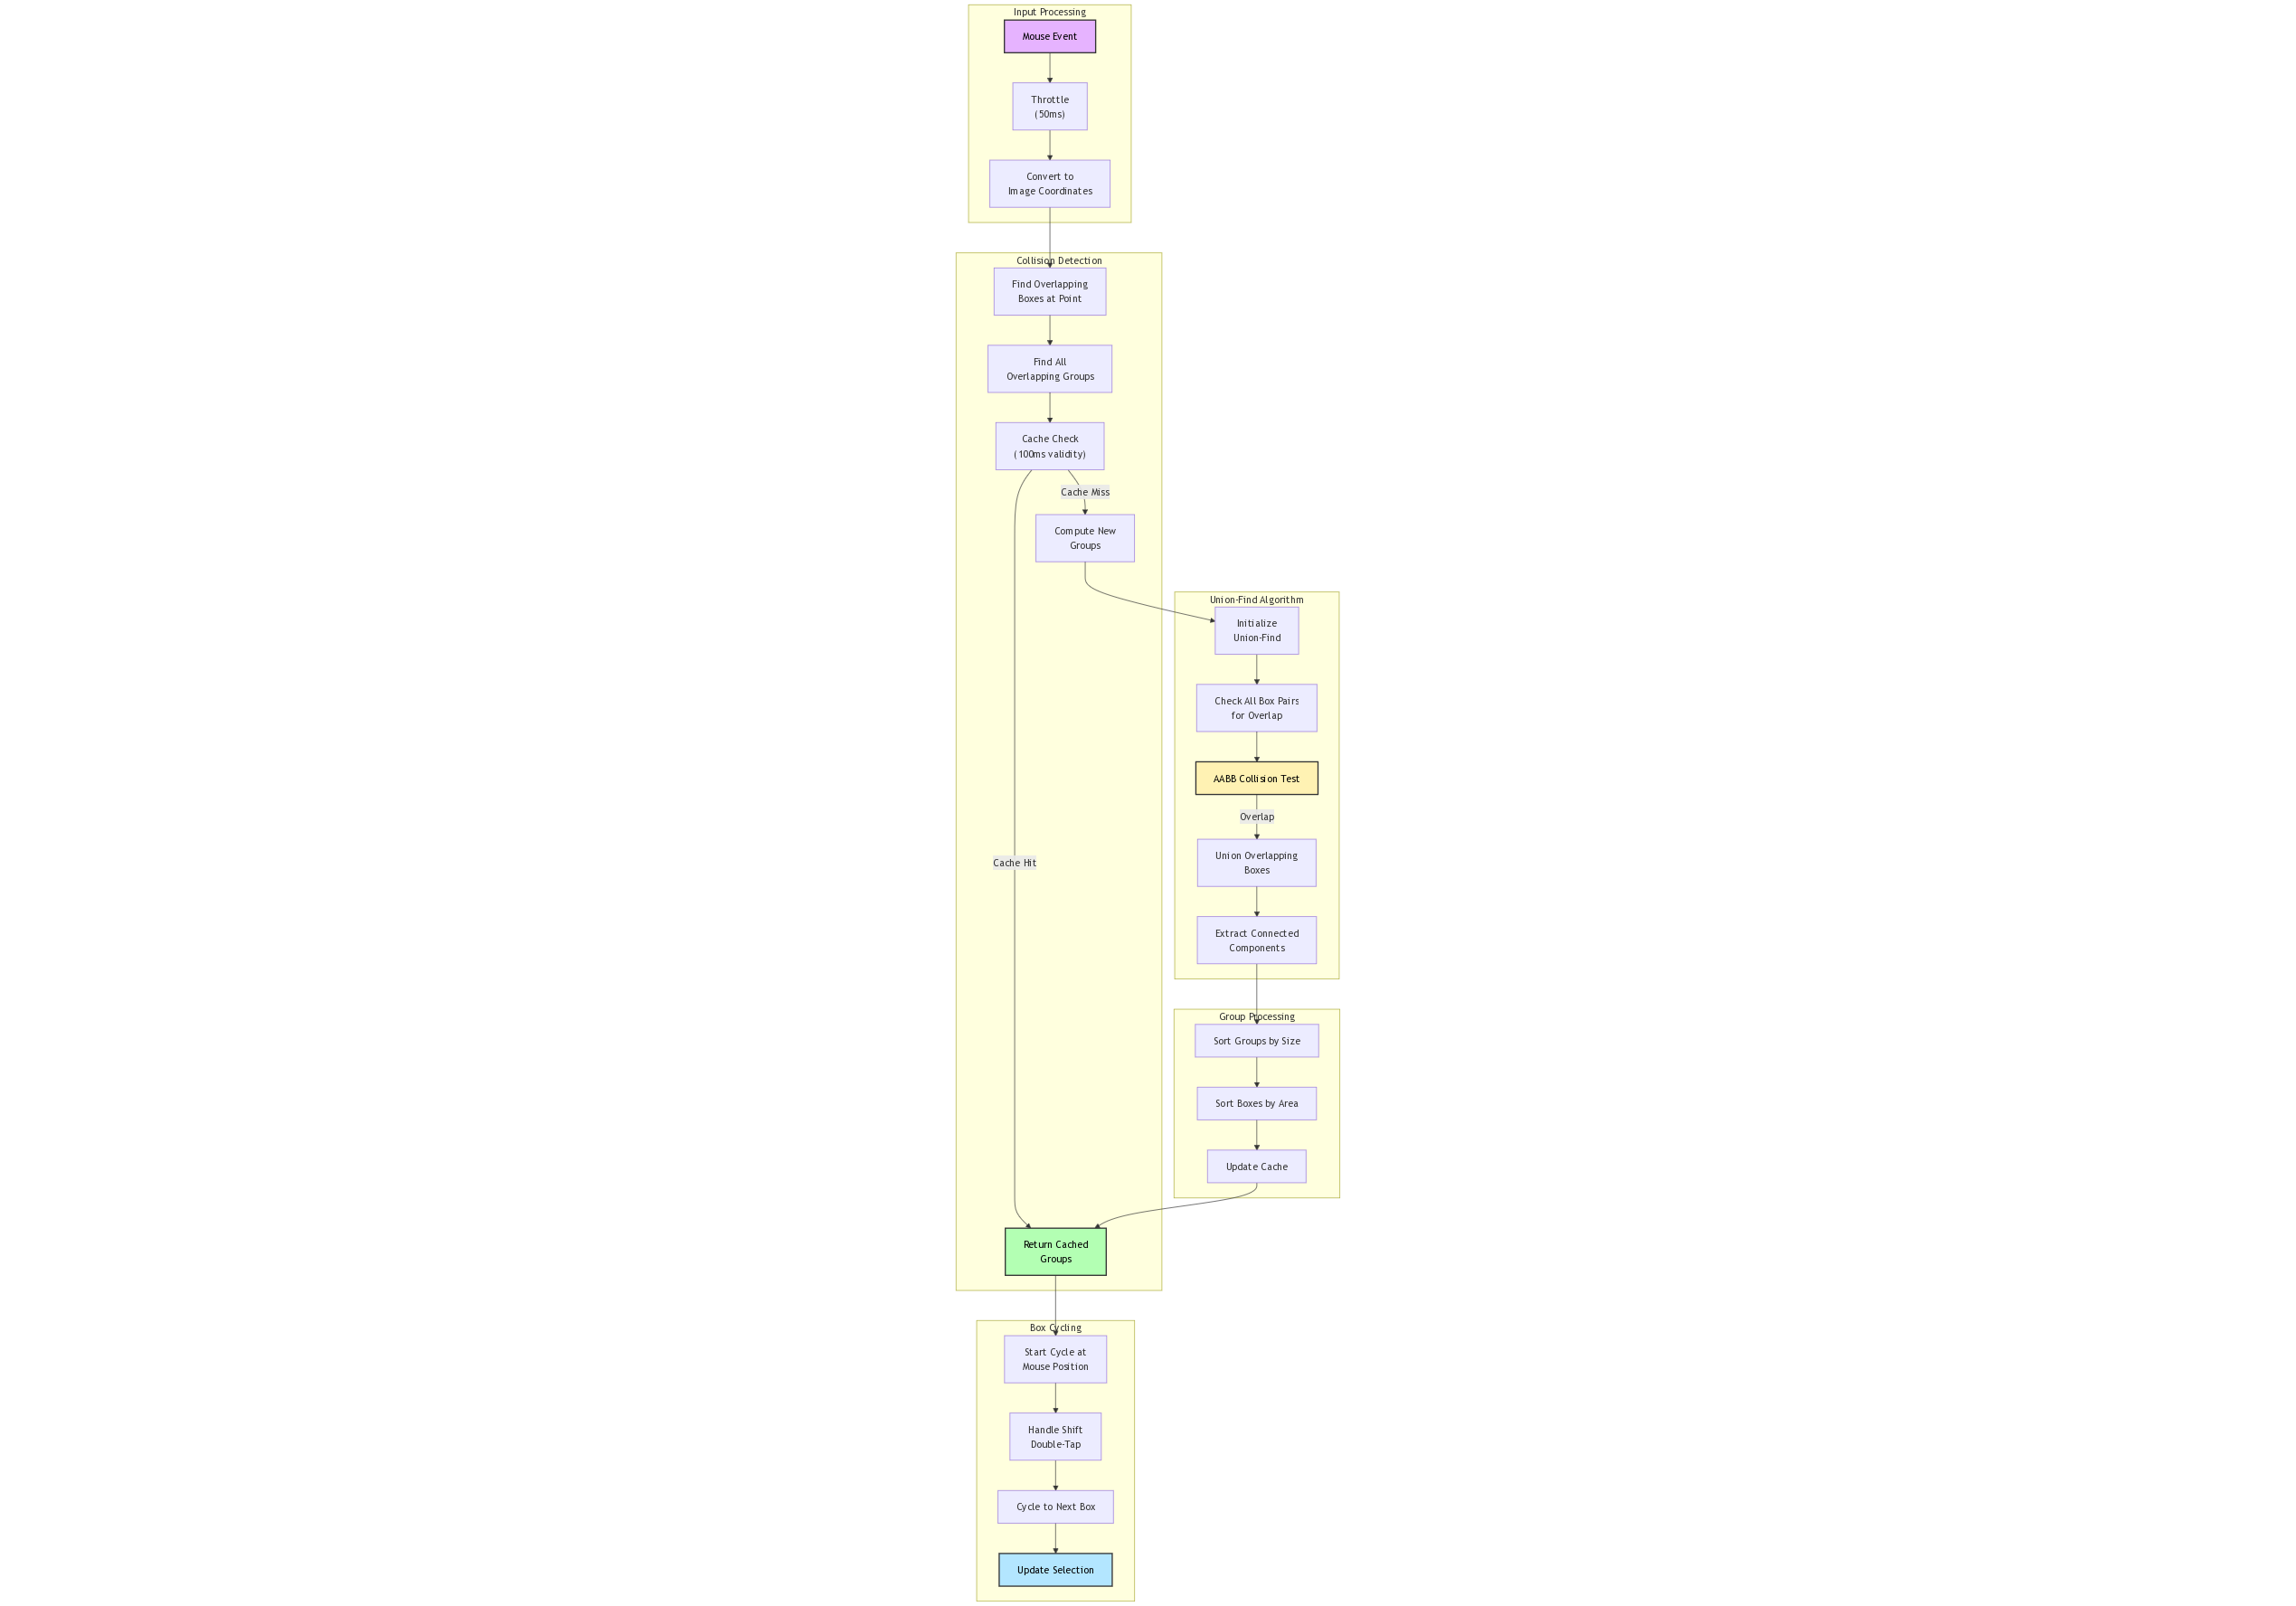
\includegraphics[height=0.85\textheight,keepaspectratio]{BoundingBox.png}
\caption{NEXUS System Architecture and Data Flow}
\label{fig:nexus_architecture}
\end{figure}

\subsection{Integration Details}
The NEXUS system operates through five distinct phases as illustrated in 
Figure~\ref{fig:nexus_architecture}:

\begin{enumerate}
    \item \textbf{Input Processing}: Mouse events are captured and throttled at 50ms intervals to maintain system responsiveness. The input coordinates are transformed from screen space to image space to identify which boxes are directly under the cursor.

    \item \textbf{Collision Detection}: The system continuously maintains a cached, comprehensive map of all overlapping bounding boxes using the Union-Find algorithm. The boxes identified under the cursor from the input processing phase are then used to select the correct, complete overlap group from this map for interactive cycling.

    \item \textbf{State Management}: When the user cycles through a group, the change in the selected box triggers state updates through SolidJS signals. This ensures the application's core state is always consistent.

    \item \textbf{UI Updates}: The reactive system, listening to state changes, automatically propagates updates to affected components. This includes visually highlighting the currently selected box while maintaining consistent frame rates.

    \item \textbf{Event Emission}: The selection change is broadcast via a type-safe event system, allowing other decoupled application components to respond to the newly selected box.
\end{enumerate}

\subsection{Workload Characteristics}
Annotation scenarios in YipYap typically involve 10 to 50 concurrent bounding boxes, with occasional peaks of up to 100 boxes. The NEXUS system is optimized for this specific workload range.

Future studies may evaluate NEXUS against other collision detection systems using workloads and interaction patterns common in image labeling.

\subsection{Key Achievements}
The integration of NEXUS into YipYap yielded several key improvements:
\begin{itemize}
    \item Sub-3ms response times for typical workloads.
    \item Seamless integration with reactive state management.
    \item Efficient memory usage via optimized data structures.
    \item A reliable, type-safe event system for communication.
\end{itemize}

\section{Experimental Results}
The performance of NEXUS was evaluated through a series of benchmarks designed to simulate real-world annotation scenarios.

\begin{table}[H]
\caption{NEXUS Performance Benchmarks - Empirical Results}
\label{tab:benchmarks}
\begin{center}
\begin{tabular}{lrrrr}
\toprule
Operation & Frequency (Hz) & Mean Time & P99 Time & RME \\
\midrule
Initialize (10 boxes) & 1,220.01 & 0.82ms & 1.65ms & ±2.33\% \\
Initialize (50 boxes) & 214.82 & 4.66ms & 5.81ms & ±1.92\% \\
Initialize (100 boxes) & 68.68 & 14.56ms & 17.15ms & ±2.86\% \\
\midrule
Overlap Detection (10 boxes) & 479.71 & 2.08ms & 2.73ms & ±1.25\% \\
Overlap Detection (50 boxes) & 93.98 & 10.64ms & 12.26ms & ±1.03\% \\
Overlap Detection (100 boxes) & 45.07 & 22.19ms & 23.58ms & ±1.31\% \\
\midrule
Box Cycling (10 overlapping boxes) & 462.24 & 2.16ms & 3.03ms & ±1.49\% \\
Box Cycling (50 overlapping boxes) & 94.48 & 10.58ms & 11.14ms & ±0.44\% \\
\bottomrule
\end{tabular}
\end{center}
\end{table}

\subsection{Scalability Analysis}
Our empirical benchmarks demonstrate NEXUS's excellent scalability characteristics across varying workloads. The system maintains sub-3ms response times for typical annotation scenarios (10-50 boxes) and exhibits predictable performance degradation as box count increases.

Performance scaling analysis reveals:
\begin{itemize}
    \item \textbf{Initialization Scaling}: Shows approximately O(n log n) complexity, with 10-box scenarios achieving 1,220 Hz (0.82ms) and 100-box scenarios maintaining 68.7 Hz (14.6ms)
    \item \textbf{Overlap Detection Scaling}: Demonstrates consistent O(n²) behavior with efficient early termination, ranging from 479.7 Hz for 10 boxes to 45.1 Hz for 100 boxes
    \item \textbf{Box Cycling Performance}: Maintains high throughput even with complex overlaps, achieving 462.2 Hz for 10-box and 94.5 Hz for 50-box scenarios
    \item \textbf{Low Variance}: All operations show relative margin of error below 3\%, indicating consistent performance characteristics
\end{itemize}

\subsection{Benchmark Methodology}
The benchmark protocol was designed to evaluate performance across a range of scenarios:
\begin{enumerate}
    \item \textbf{Initialization}: Started with random, non-overlapping boxes to set a baseline.

    \item \textbf{Controlled Overlap}: Specific overlap densities (20\%, 50\%, 80\%) were created by resizing and repositioning boxes.

    \item \textbf{Real-time Interaction Simulation}: Measures box cycling performance under conditions simulating actual user interaction patterns.
\end{enumerate}

\subsection{Algorithm Comparison Methodology}
Direct benchmarks against other algorithms were not performed for several strategic reasons:

\begin{enumerate}
    \item \textbf{Workload-Specific Design}: NEXUS is tailored for dynamic bounding box tasks. General algorithms have unneeded overhead for our use case. We focused on perfecting our main interaction model.

    \item \textbf{Complexity}: Benchmarking other complex collision systems was beyond the project's scope. The focus was on delivering a performant feature in our existing architecture.

    \item \textbf{Predictability}: Union-Find offers predictable, near-constant time complexity. This is vital for a smooth UX, as other methods can have performance cliffs.
\end{enumerate}

\section{Mathematical Formulation of Box Cycling}
The interactive box cycling algorithm is defined by a series of mathematical and logical operations that transform user input into a predictable and intuitive navigation experience.

Let $B = \{b_1, b_2, \ldots, b_n\}$ be the set of all bounding boxes.
Let $P_c = (x_c, y_c)$ be the cursor position in image coordinates.

\subsection{Hover Detection and Candidate Selection}
First, we identify the set of boxes directly under the cursor, $B_{cand} \subseteq B$. A box $b_i = (x_i, y_i, w_i, h_i)$ is a candidate if the cursor is within its bounds:
\begin{equation}
    b_i \in B_{cand} \iff (x_i \le x_c \le x_i + w_i) \land (y_i \le y_c \le y_i + h_i)
\end{equation}

The candidate set is then sorted by area in ascending order:
\begin{equation}
    B'_{cand} = \text{sort}(B_{cand}, \text{key=area})
\end{equation}

\subsection{Cycle Group Determination}
Let $G = \{G_1, G_2, \ldots, G_m\}$ be the set of all overlap groups (connected components) pre-computed by the Union-Find algorithm.

The cycle group, $G_{cycle}$, is determined by finding the group associated with the smallest-area candidate box, $b'_{cand,1}$:
\begin{equation}
    G_{cycle} = G_j \quad \text{such that} \quad b'_{cand,1} \in G_j
\end{equation}
If $B'_{cand}$ is empty, no cycle group is selected.

\subsection{User-Initiated Cycling}
The user initiates cycling through $G_{cycle}$, which is pre-sorted by area. Let the currently selected box be $b_{current}$. The next box, $b_{next}$, is determined by a double-tap of the Shift key:
\begin{equation}
    \text{index}_{next} = (\text{index}(b_{current}, G_{cycle}) + 1) \pmod{|G_{cycle}|}
\end{equation}
\begin{equation}
    b_{next} = G_{cycle}[\text{index}_{next}]
\end{equation}
The `index()` function returns the 0-based position of $b_{current}$ in the sorted group $G_{cycle}$. The modulo operator ensures the cycle wraps around to the beginning.

\section{Novelty and Contributions}
This work makes several contributions to the field of interactive image annotation systems:
\begin{enumerate}
    \item \textbf{Application-Specific Optimization}: While connected components analysis for geometric objects is established in computational geometry literature, NEXUS provides a tailored implementation optimized specifically for real-time image annotation workflows. The system achieves sub-3ms response times through careful engineering choices including strategic caching, event throttling, and reactive state management integration.

    \item \textbf{Interactive Navigation Interface}: The shift-key double-tap cycling mechanism provides an intuitive method for users to navigate through overlapping annotation groups. This interaction pattern addresses the practical challenge of selecting obscured annotations in dense labeling scenarios.

    \item \textbf{Production System Integration}: NEXUS demonstrates effective integration of spatial clustering algorithms within a modern reactive web framework (SolidJS), providing empirical performance data for annotation workloads typical in production environments (10-100 concurrent bounding boxes).

    \item \textbf{Empirical Performance Characterization}: The paper provides comprehensive benchmarking data showing consistent performance characteristics across varying workload sizes, with detailed analysis of initialization, overlap detection, and cycling operations.
\end{enumerate}

These contributions enable efficient user interaction with overlapping annotations while maintaining responsive performance in production annotation systems.

\begin{sloppypar}
\section{Conclusion}
NEXUS demonstrates exceptional performance as a real-time collision detection system for interactive image annotation applications. The system's integration into the YipYap platform validates its effectiveness in production environments, achieving sub-3ms response times for typical annotation scenarios while maintaining consistent performance characteristics across varying workloads.

Key contributions of this work include:
\begin{itemize}
    \item An optimized implementation of Union-Find algorithms tailored for annotation workflows
    \item A scalable, cache-aware architecture for dynamic collision detection
    \item Empirical validation of sub-3ms performance in a production environment
\end{itemize}
\end{sloppypar}

\bibliographystyle{IEEEtran}
\begin{thebibliography}{99}
\bibitem{tarjan} R. E. Tarjan and J. van Leeuwen, "Worst-case analysis of set union algorithms," J. ACM, vol. 31, no. 2, pp. 245-281, 1984.
\bibitem{aabb} G. van den Bergen, "Collision Detection in Interactive 3D Environments," Morgan Kaufmann Publishers, 2003.
\bibitem{phraseclick2020}
Ding, H., Cohen, S., Price, B., \& Jiang, X. (2020). PhraseClick: Toward Achieving Flexible Interactive Segmentation by Phrase and Click. In Computer Vision -- ECCV 2020 (pp. 417-435). Springer, Cham.

\bibitem{focalclick2022}
Chen, X., Zhao, Z., Zhang, Y., Duan, M., Qi, D., \& Zhao, H. (2022). FocalClick: Towards Practical Interactive Image Segmentation. In Proceedings of the IEEE/CVF Conference on Computer Vision and Pattern Recognition.

\end{thebibliography}

\end{document} 